%\documentclass[a4paper]{article}
%\usepackage{graphicx,placeins}
%\usepackage{epsfig}
%\usepackage{comment}
%\usepackage{amsmath,amsthm}
%\usepackage{xspace}
%\usepackage[colorlinks=true,citecolor=blue]{hyperref}
%\usepackage[acronym,nonumberlist,nogroupskip]{glossaries}
%\usepackage{showlabels}
%\usepackage{titlesec}
%\setcounter{secnumdepth}{4}
%\titleformat{\paragraph}
%{\normalfont\normalsize\bfseries}{\theparagraph}{1em}{}
%\titlespacing*{\paragraph}
%{0pt}{3.25ex plus 1ex minus .2ex}{1.5ex plus .2ex}
%
%\newcommand{\etal}{{\it et~al.}\ }
%\newcommand{\ie}{{\it i.e.}\ }
%\newcommand{\eg}{{\it e.g.}\ }
%\newcommand{\Ito}{It\^{o} }
%\newcommand{\tsing}{t_{\text{singular}}}
%\newcommand{\gest}{g_{\text{est}}}
%\newcommand{\eq}{\hspace{-.15cm}=\hspace{-.15cm}}
%
%\newcommand{\ave}[1]{\left\langle#1 \right\rangle}
%\newcommand{\dist}{\,{\buildrel d \over =}\,}
%\newcommand{\mut}{\tilde{\mu}}
%\newcommand{\sigmat}{\tilde{\sigma}}
%\newcommand{\var}{\text{var}}
%\newcommand{\stdev}{\text{stdev}}
%
%\newcommand{\rex}{r_{\ave{}}}
%\newcommand{\rt}{r_{t}}
%
%\newcommand{\gt}{g_{t}}
%\newcommand{\gex}{g_{\ave{}}}
%
%
%\newcommand{\elabel}[1]{\label{eq:#1}}
%\newcommand{\eref}[1]{(Eq.~\ref{eq:#1})}
%\newcommand{\Eref}[1]{Equation~(\ref{eq:#1})}
%
%\newcommand{\ceref}[2]{(\ref{eq:#1}#2)}
%
%\newcommand{\tlabel}[1]{\label{tab:#1}}
%\newcommand{\tref}[1]{(Table~\ref{tab:#1})}
%
%\newcommand{\flabel}[1]{\label{fig:#1}}
%\newcommand{\fref}[1]{Fig.~\ref{fig:#1}}
%\newcommand{\Fref}[1]{Figure ~\ref{fig:#1}}
%
%\newcommand{\seclabel}[1]{\label{section:#1}}
%\newcommand{\secref}[1]{Sec.~\ref{section:#1}}
%\newcommand{\Secref}[1]{Section~\ref{section:#1}}
%
%\newcommand{\OP}[1]{{\bf @@@OP: #1 @@@}}
%\renewcommand{\AA}[1]{{\bf ===AA: #1 ===}}
%
%\newcommand{\be}{\begin{equation}}
%\newcommand{\ee}{\end{equation}}
%\newcommand{\bea}{\begin{eqnarray}}
%\newcommand{\eea}{\end{eqnarray}}
%\newcommand{\bc}{\begin{center}}
%\newcommand{\ec}{\end{center}}
%\newcommand{\prob}[1]{\mathcal{P}\left(#1\right)}
%\newcommand{\D}{\Delta}
%\newcommand{\PDF}{\mathcal{P}}
%\newcommand{\nn}{\nonumber}
%
%\newcommand{\definition}[1]{\vspace{.2cm} {\bf \underline{Definition} #1} \vspace{.2cm}}

\newpage

\section{Populations}
{\it 
The previous chapter developed a model of individual behaviour based on an
assumed dynamic imposed on wealth. If we know the stochastic process that describes
individual wealth, then we also know what happens at population level -- each individual
is represented by a realisation of the process, and we can compute 
the dynamics of wealth distributions. We answer questions about inequality and poverty in
our model economy. It turns out that our decision criterion generates interesting emergent
behaviour -- cooperation, the sharing and pooling of resources, is often time-average 
growth optimal. This provides answers to the puzzles of why people cooperate, why there 
is an insurance market, and why we see socio-economic structure from the formation of 
firms to nation states with taxation and redistribution systems.}
\newpage

\subsection{Every man for himself}
\seclabel{Every_man}

We have seen that risk aversion constitutes optimal behaviour under the assumption 
of multiplicative wealth growth and over time scales that are long enough for systematic 
trends to be significant. In this chapter we will continue to explore our null model, 
GBM. By ``explore'' we mean that we will let the model generate its world -- if 
individual wealth was to follow GBM, what kind of features of an economy would emerge? 
We will see that cooperation and the formation of social structure also constitute 
optimal behaviour.

GBM is more than a random variable, it's a stochastic process, \ie a set of trajectories 
$x(t)$ or  a family of random variables parameterized by $t$, depending on how we 
prefer to look at it.  Both perspectives are informative in the context of economic modelling
-- from the set of trajectories we can judge what is likely to happen to an individual, 
\eg by following an individual trajectory for a long time, and the PDF of the random 
variable $x(t^*)$ at some fixed value of $t^*$ is the wealth distributed in our model. 

We use the term wealth distribution to refer to the density function 
$\PDF_x(x)$ (not to the process of distributing wealth among people). This can be 
interpreted as follows: if I select a random individual (each individual with uniform probability 
$\frac{1}{N}$), the probability of the selected individual 
having wealth greater than $x$ is given by the CDF $F_x(x)=\int_x^\infty ds \PDF_x(s)$.
In a large population of $N$ individuals, $\D x \PDF_x(x)N$ is the approximate 
number of individuals who have wealth near $x$. 
Thus, a broad wealth distribution with heavy tails indicates greater wealth inequality. 

\underline{Examples:}
\begin{itemize}
\item Under perfect equality everyone would have the same, meaning that the wealth
distribution would be a Dirac delta function centered at the mean of $x$, that is
\be
\PDF_x(x)=\delta(x-\ave{x}_N);
\ee
\item
Maximum inequality would mean that one individual owns everything
and everyone else owns nothing, that is
\be 
\PDF_x(x)=\frac{N-1}{N}\delta(x-0)+\frac{1}{N}\delta(x-N\ave{x}_N).
\ee
\end{itemize}

\subsubsection{Log-normal wealth distribution}
\seclabel{Log-normal_wealth}
GBM is log-normally distributed. If each individual's wealth follows GBM,
\be
dx=x(\mu dt + \sigma dW),
\elabel{GBM}
\ee
with solution 
\be
x(t) = x_0 \exp\left[\left(\mu-\frac{\sigma^2}{2}\right)t + \sigma W(t)\right],
\ee
then we will observe a log-normal wealth distribution at each moment in time:
\be
\ln x(t) \sim \mathcal{N}\left(\ln x_0 + \left(\mu - \frac{\sigma^2}{2}\right)t, \sigma^2 t\right).
\elabel{lognormal}
\ee


We notice that the variance of $\ln x$ increases linearly in time -- 
we will develop an understanding of this fact shortly. As we will see 
(though we cannot conclude this yet), it indicates that any meaningful 
measure of inequality will grow over time in our simple model. 
To see what kind of a wealth distribution \eref{lognormal} is, it is worth 
spelling out the lognormal PDF
\be
\PDF(x)=\frac{1}{x\sqrt{2\pi \sigma^2t}}\exp\left(-\frac{[\ln(x)-(\mu-\frac{\sigma^2}{2})t]^2}{2\sigma^2 t} \right).
\elabel{PDFx}
\ee

INSERT PROPERTIES OF GBM DISTRIBUTION HERE (note that lognormal is an insufficient description of the distribution of a GBM - the time-dependence of the random variable must be included)

It is a well-established empirical observation \cite{Newman2005} that the upper tails of 
real wealth distributions tend to look more like a power law than a log-normal. Our trivial model does not
strictly reproduce this feature, but it is instructive to compare the lognormal distribution
to a power-law distribution. A power law PDF has the aymptotic form 
\be
\PDF_x(x)= x^{-\alpha},
\elabel{power_law}
\ee
for large arguments $x$. This implies that the logarithm of the PDF is proportional 
to the logarithm of its argument, $\ln \PDF_x(x) = -\alpha \ln x$. Plotting
one against the other will yield a straight line, the slope being the exponent $-\alpha$. 

Determining whether an empirical observation is consistent with such behaviour 
is difficult because the behaviour is to be observed in the tail (large $x$) where data are
by definition sparse. A quick-and dirty way of checking for possible power-law 
behavior is to plot an empirical PDF against its argument on log-log scales, 
look for a straight line, and measure the slope. However, plotting any distribution on any 
type of scales results in some line. It may not be a straight line but it will have some slope 
everywhere. For a known distribution (power law or not) we can interpret this slope 
as a local apparent power-law exponent. 

What is the local apparent power-law exponent of a log-normal wealth distribution near the 
expectation value $\ave{x}$, \ie in the upper tail where approximate power law behavior
has been observed empirically? The logarithm of \eref{PDFx} is
\bea
\ln \PDF(x)&=&-\ln x\sqrt{2\pi \sigma^2t} -\frac{([\ln(x)-(\mu-\frac{\sigma^2}{2})t]^2}{2\sigma^2 t}\\
&=&-\ln x -\frac{\ln (2\pi \sigma^2t)}{2} - \frac{(\ln(x)^2+[(\mu-\frac{\sigma^2}{2})t]^2-2(\mu-\frac{\sigma^2}{2})t \ln x}{2\sigma^2 t}
\eea
Collecting terms in powers of $\ln x$ we find
\be
\ln \PDF(x)=[\ln x]^2 \times\frac{-1}{2\sigma^2 t}  + \ln x \times \left(-\frac{3}{2}+\frac{\mu}{\sigma^2} \right) -\frac{\ln(2 \pi\sigma^2 t)}{2}-\frac{[(\mu-\frac{\sigma^2}{2})t]^2}{2\sigma^2 t}
\ee
with local slope, \ie apparent exponent,
\be
\frac{d\ln \PDF(x)}{d \ln x}=-\frac{\ln x}{\sigma^2 t}  - \frac{3}{2}+\frac{\mu}{\sigma^2}.
\ee
If the first term is small compared to the others, this distribution will look like a power law when
plotted on double-logarithmic scales. We don't believe that the empirically observed power laws
are merely a manifestation of this mathematical feature. Important real-world  mechanisms 
that broaden real wealth distributions, \ie concentrate wealth, are missing from the 
null model. However, it is interesting that the trivial model of GBM chimes with so many qualitative 
features of empirical observations. 

\subsubsection{Inequality measure from two growth rates}
\seclabel{Inequality_measure}
In the case of GBM we have just seen how to 
compute the exact full wealth distribution $\PDF$. This is intersting, but
we often only want summary measures of the distribution. A distributional property of particular 
interest to economists is inequality. How much inequality is there in a distribution like \eref{lognormal}, 
and in what sense does this quantity increase in time under GBM as we have pointed out?
Clearly, we should quantify ``inequality''. In this section we develop a natural way of measuring it, 
which makes use of the two growth rates we identified for the non-ergodic process. We will see 
that a particular inequality measure, known to economists as
Theil's second index of inequality \cite{Theil1967}, is the difference
between typical wealth (that grows at the time-average growth rate) and average wealth 
(that grows at the ensemble-average growth rate) in our model. Thus, the difference between
the time average and ensemble average, the essence of ergodicity breaking, 
fundamentally drives  the dynamics of inequality.

The two limits of inequality are easily identified: minimum inequality means that everyone 
has the same wealth, and maximum inequality means that one individual has all the 
wealth and everyone else has nothing (this assumes that wealth cannot become 
negative). Quantifying inequality in any other distribution is reminiscent of the gamble 
problem. Recall that for gambles we wanted make statements of the type ``this gamble 
has more desirability than that gamble''. We did this by collapsing a distribution to a 
scalar. Depending on the question that was being asked 
the appropriate way of collapsing the distribution and the resulting scalar can be different 
(the scalar relevant to an insurance company may not be relevant to an individual). 
In the case of inequality we also have a distribution -- the wealth distribution -- and we 
want to make statements of the type ``this distribution has more inequality than that 
distribution''. Again, this is done by collapsing the distribution to a scalar, and again 
many different choices of collapse and resulting scalar are possible. The Gini 
coefficient is a particularly well-known scalar of this type, the 80/20 ration is another, 
and many other measures exist.

In this context the expectation value is an important quantity. 
%Allowing initial wealth, 
%$x_0$, to be a random variable, the mean of the wealth distribution \eref{lognormal} is
%\be
%\ave{x(t)}=\ave{x_0}e^{\mu t}.
%\ee
For instance, if everyone has the same wealth, everyone will own the average $\forall i, x_i=\ave{x}_N$,
which converges to the expectation value for large $N$. Also, whatever the distribution 
of wealth, the total wealth is $N\ave{x}_N$ which converges to $N\ave{x}$. The growth 
rate of the expectation value, $\gex$, thus tells us how fast the average wealth and the 
total population wealth grow with probability one in a large ensemble. The time-average 
growth rate, $\gt$, tells us how fast an individual's wealth grows with probability one in 
the long run. If the typical individual's wealth grows at a lower rate than the 
expectation value of wealth then there must be a-typical individuals with very large 
wealth that account for the difference. This suggests the following measure of 
inequality.

\definition{
inequality $J(t)$, is the quantity that grows in time at the rate of the 
difference between expectation-value and time-average growth rates,
%The inequality present in the distribution does not depend on absolute 
%wealth levels, which is one of four criteria that together define so-called ``relative inequality 
%measures'' \cite[p.~139]{Sen1997}. It is convenient to divide everyone's wealth by the 
%common factor $\ave{x}$ and focus on the rescaled wealth,
%\be
%y \equiv \frac{x}{\ave{x}} = \frac{xe^{-\mu t}}{\ave{x_0}},
%\elabel{ydef}
%\ee
%This is done purely for mathematical convenience and does not affect any reasonable measure of inequality.
%The SDE for $y$ is obtained by applying \Ito's version of the chain rule for SDEs: 
%\bea
%dy &=& \frac{\partial y}{\partial t}\,dt + \frac{\partial y}{\partial x}\,dx + \frac{1}{2} \frac{\partial^2 y}{\partial x^2} \,dx^2 \\
%&=& -\mu y\,dt + \frac{y}{x}\,dx \elabel{ysde} \\
%&=& y\sigma\,dW.
%\eea
%The rescaled wealth remains distributed as a continually-broadening lognormal but it no longer depends on the drift,
%\be
%\ln y(t) \sim \mathcal{N}\left(-\frac{\sigma^2 t}{2}, \sigma^2 t\right).
%\elabel{y_lognorm}
%\ee
%It has constant unit mean, which is trivially shown by noting that
%\be
%\ave{y} = \ave{\frac{x}{\ave{x}}} = 1.
%\elabel{ymean}
%\ee
\be
\frac{dJ}{dt}=\gex-\gt.
\elabel{dJ}
\ee
\Eref{dJ} defines the dynamic of inequality, and inequality itself is found by 
integrating over time
\be
J(t)=\int_0^t ds [\gex(s)-\gt(s)].
\elabel{J}
\ee
}

This definition may be used for dynamics other than
GBM. Whatever the wealth dynamic, typical minus average growth rates are informative of the
dynamic of inequality. Within the GBM framework we can write down the two growth rates 
explicitly and find 
\be
\frac{dJ}{dt}=\frac{d \ln \ave{x}}{dt}-\frac{d \ave{\ln x}}{dt}.
\elabel{J_dyn}
\ee
Integrating over time
\be
J(t)=\ln \ave{x}-\ave{\ln x},
\ee
which is known as the mean logarithmic deviation (MLD) or Theil's second index of inequality \cite{Theil1967}. 
This is rather remarkable. Our general inequality measure, \eref{J}, evaluated 
for the specific case of GBM, turns out to be a well-known measure of inequality that 
economists identified independently, without considering non-ergodicity and ensemble 
average and time average growth rates. Merely by insisting of measuring inequality well,
Theil implicitly used the GBM model!

The expectation value $\ave{\ln x}=\ln x_0 + \left(\mu - \frac{\sigma^2}{2}\right)t$ is
given by \eref{lognormal}. It differs from the logarithm of the expectation value, 
$\ave{\ln x}\neq \ln\ave{x}$, which we now compute. In order to do this we introduce 
a useful trick that will come in handy again in \secref{Wealth_tax} (the general 
procedure is described in \cite[Chapter 4.2]{KloedenPlaten1992}): to compute
moments, $\ave{x^n}$, of stochastic differential equations for $x$,  like 
\eref{GBM}, we find solvable ordinary differential equations for the moments. 
For the first moment we do this simply by taking expectations of both sides of \eref{GBM}.
The noise term disappears, and we turn the SDE for $x$ into an ODE for $\ave{x}$
\bea
\ave{dx}&=&\ave{x(\mu dt + \sigma dW)}\\
d\ave{x}&=&\ave{x} \mu dt + \sigma \overbrace{\ave{dW}}^{=0}\\
&=&\ave{x} \mu dt.
\eea
This is a (very simple) first order linear differential equation for 
the first moment (\ie the expectation value) of $x$. Its solution is
\be
\ave{x}=\ave{x_0} \exp(\mu t)
\elabel{exp_x}
\ee
so that $\ln\ave{x}=\ln \ave{x_0} + \mu t$.  Now we can carry out the differentiations
on the RHS of \eref{J_dyn} and find the Theil inequality as a function of time
\be
J(t)=J(0)+\frac{\sigma^2}{2} t.
\ee
Inequality increases indefinitely. This result implies an evolution towards wealth condensation. Wealth condensation 
means that a single individual will own a non-zero fraction of the total wealth in the 
population in the limit of large $N$, see \eg \cite{BouchaudMezard2000}. In the 
present case an arbitrarily large share of total wealth will be owned by an arbitrarily 
small share of the population. 


Over the decades, economists have arrived at many inequality measures, and have drawn 
up a list of conditions that particularly useful measures of inequality satisfy. Such measures
are called ``relative measures'' \cite[Appendix 4]{Sen1997}, and $J$ is one of them. One of the conditions is that inequality measures
should not change when $x$ is divided by the same factor for everyone. Since we are primarily 
interested in inequality in this section it is useful to remove absolute wealth levels from the
analysis and study an object called the rescaled wealth.

\definition{
The rescaled wealth, 
\be
y=\frac{x}{\ave{x}_N},
\elabel{rescaled}
\ee
is the proportion of the population-average wealth owned by an individual.}

This quantity is useful, for instance because its numerical value does not 
depend on the currency used, it is a dimensionless number. 
Thus if my rescaled wealth, $y=1/2$, this means that my wealth is half the 
average wealth, irrespective of whether I measure wealth in Kazakhstani Tenge 
or in Swiss Francs. \Eref{J_dyn}, may be expressed in 
terms of $y$ as $\frac{dJ}{dt}=-\frac{d\ave{\ln y}}{dt}$. 

%One way of seeing this is to calculate the fraction of 
%the population whose wealths are less than the mean. From \eref{y_lognorm} we 
%define a new variable, z, whose distribution is the standard normal:
%\be
%z \equiv \frac{\ln y + \sigma^2t/2}{\sigma t^{1/2}} \sim \mathcal{N}(0,1).
%\ee
%We are interested in the mass of the distribution with $\ln y<0$, which is simply
%\be
%\prob{z<\frac{\sigma t^{1/2}}{2}} = \Phi\left(\frac{\sigma t^{1/2}}{2}\right),
%\ee
%where $\Phi$ is the standard normal cdf. This fraction tends to one as $t\to\infty$.

\subsection{Sums of lognormals and the random energy model}
\seclabel{REM}

\subsubsection{Introduction -- why study GBM?}
The basic phenomenon of self-reproduction occurs from the 
smallest chemical compound capable of building copies of itself to arguably the most complex 
known social system, namely the global economy. Not only is the economy made by humans 
who self-reproduce and whose cells self-reproduce but capitalism itself taps into the power of 
self-reproduction: capital means resources which can be deployed in order to 
generate resources, which can be deployed in order\dots. Realism usually requires models that include noise, to account for the multitude of effects not explicitly modelled. GBM is a simple, intuitive, and analytically tractable model of noisy multiplicative growth. 
A deep understanding of this basic model of self-reproduction is crucial and only in the last few decades have 
we achieved this. 

A quantity, $x$, of self-reproducing resources (such as biomass or capital) follows GBM if it evolves over time, $t$, according to the \Ito stochastic differential equation,
\be
dx=x(\mu dt+\sigma dW_t).
\elabel{GBM}
\ee
$dt$ denotes the infinitesimal time increment and $dW_t$ the infinitesimal increment in a Wiener process, which is a normal variate with $\ave{dW_t}=0$ and $\ave{dW_t dW_s}=\delta(t-s) dt$. $\mu$ and $\sigma$ are constant parameters called the drift and volatility. Put simply, relative changes in resources, $dx/x$, are assumed to be drawn independently from a stationary normal distribution at each time step. \eref{GBM} represents the continuous-time limit of this process. Its solution,
\be
x(t)=x(0)\exp\left[\left(\mu-\frac{\sigma^2}{2}\right) t+\sigma W(t)\right],
\elabel{GBM_sol}
\ee
yields exponential growth at a noisy rate. Hereafter, we shall assume $x(0)=1$ and neglect it, except where retaining it is illustrative. The distribution of $x(t)$ is a time-dependent log-normal,
\be
\ln(x(t)) \sim \mathcal{N}\left( \left(\mu-\frac{\sigma^2}{2}\right)t,\, \sigma^2 t \right),
\ee
whose mean, median, and variance grow (or decay) exponentially in time:
\bea
\ave{x(t)} &=& \exp(\mu t); \elabel{mean_x}\\
\text{median}(x(t)) &=& \exp[(\mu-\sigma^2/2)t]; \elabel{median_x}\\
\text{var}(x(t)) &=& \exp(2\mu t)[\exp(\sigma^2t)-1]. \elabel{var_x}
\eea

GBM is a standard model in finance for self-reproducing quantities such as stock prices. Since relative changes are modelled as normal variates, the central limit theorem means that GBM is an attractor process for a large class of multiplicative dynamics. Any quantity whose relative changes are random variables with finite mean and variance will behave 
like a GBM after a sufficiently long time. We work with GBM because it is standard and general. It exemplifies important qualitative and universal features
of multiplicative growth.

Specifically, we are interested in GBM as a model of economic resources, owned by some entity. We will think of $x$ as measured in currency units, such as dollars.

\subsubsection{Non-ergodicity of GBM}
The non-ergodicity of this growth process
manifests itself in an intriguing way as a difference between the growth of the expectation
value of $x$ and the growth of $x$ over time. Imagine a world where people's wealth 
follows \eref{GBM}. In such a world each person's wealth grows exponentially at rate
\be
g_t=\mu-\sigma^2/2
\elabel{gt}
\ee
with probability 1 if we observe the person's wealth for a long time.
The expectation value of each person's wealth grows exponentially at
\be
g_{\ave{}}=\mu.
\elabel{gave}
\ee
The expectation value, by definition, is the average over an ensemble of $N$ realizations of
$x$ in the limit $N\to\infty$. Important insights follow: the aggregate wealth in our model 
economy does not grow at the same rate as an individual's wealth \cite{AdamouPeters2016} (meaning that GDP may be a flawed reflection of national
economic well-being); inequality grows indefinitely \cite{BouchaudMezard2000,BermanPetersAdamou2017} (even without interactions between individuals); and 
pooling and sharing resources accelerates growth \cite{PetersAdamou2015a,Bouchaud2015}.

\subsubsection{PEAs in GBM -- a sketch\seclabel{sketch}}
The following question often emerges in applications of these results. \Eref{gt} and \eref{gave} are limiting cases ($t \to \infty$ and $N\to\infty$, respectively): what happens when time and population size are finite? In \cite{PetersKlein2013} we studied the ``partial ensemble average'' (PEA) of GBM, details of which are in \secref{prevwork}. The PEA is the sample mean of $N$ independent realisations of GBM:
\be
\ave{x(t)}_N \equiv \frac{1}{N} \sum_{i=1}^N x_i(t).
\ee
Here we sketch out some simple arguments about how this object depends on $N$ and $t$.

Considering \eref{gt} and \eref{gave} together, we expect the following tension:
\begin{enumerate}
\item[A)] for large $N$, the PEA should resemble the expectation value, $\exp(\mu t)$;
\item[B)] for long $t$, all trajectories should grow like $\exp[(\mu-\sigma^2/2)t]$.
\end{enumerate}
Situation A -- when a sample mean resembles the corresponding expectation value -- is known in statistical physics as ``self-averaging.'' A simple strategy for estimating when this occurs is to look at the relative variance of the PEA,
\be
R \equiv \frac{\text{var}(\ave{x(t)}_N)}{\ave{\ave{x(t)}_N}^2}.
\ee
To be explicit, here the $\ave{\cdot}$ and $\text{var}(\cdot)$ operators, 
without $N$ as a subscript, 
refer to the mean and variance over all possible PEAs. The PEAs themselves, taken over finite samples of size $N$, are denoted $\ave{\cdot}_N$. 
Using standard results for the mean and variance of sums of independent random variables and inserting the results in \eref{mean_x} and \eref{var_x}, we get
\be
R(N) = \frac{e^{\sigma^2 t}-1}{N}.
\ee
If $R \ll 1$, then the PEA will likely be close to its own expectation value, which is equal to the expectation value of the GBM. Thus, in terms of $N$ and $t$, $\ave{x(t)}_N\approx\ave{x(t)}$ when
\be
t < \frac{\ln N}{\sigma^2}.
\elabel{short_t}
\ee
This hand-waving tells us roughly when the large-sample (or, as we see from \eref{short_t}, short-time) self-averaging regime holds. A more careful estimate of the cross-over time in \eref{t_c} is a factor of 2 larger, but the scaling is identical.

For $t>\ln N/\sigma^2$, the growth rate of the PEA transitions from $\mu$ to its $t\to\infty$ limit of $\mu-\sigma^2/2$ (Situation B). 
Another way of viewing this is to think about what dominates the average. For early times in the process, all trajectories are close together, but as time goes by the distribution broadens exponentially. Because each trajectory contributes with the same weight to the PEA, after some time the PEA will be dominated by the maximum in the sample,
\be
\ave{x(t)}_N \approx \frac{1}{N}\max_{i=1}^N \{x_i(t)\},
\ee
as illustrated in \fref{trajectories}.
Self-averaging stops when even the ``luckiest'' trajectory is no longer close to the expectation value $\exp(\mu t)$. This is guaranteed to happen eventually because the probability for a trajectory to reach $\exp(\mu t)$ decreases towards zero as $t$ grows. Of course, this takes longer for larger samples, which have more chances to contain a lucky trajectory. 

\begin{figure}
\centering
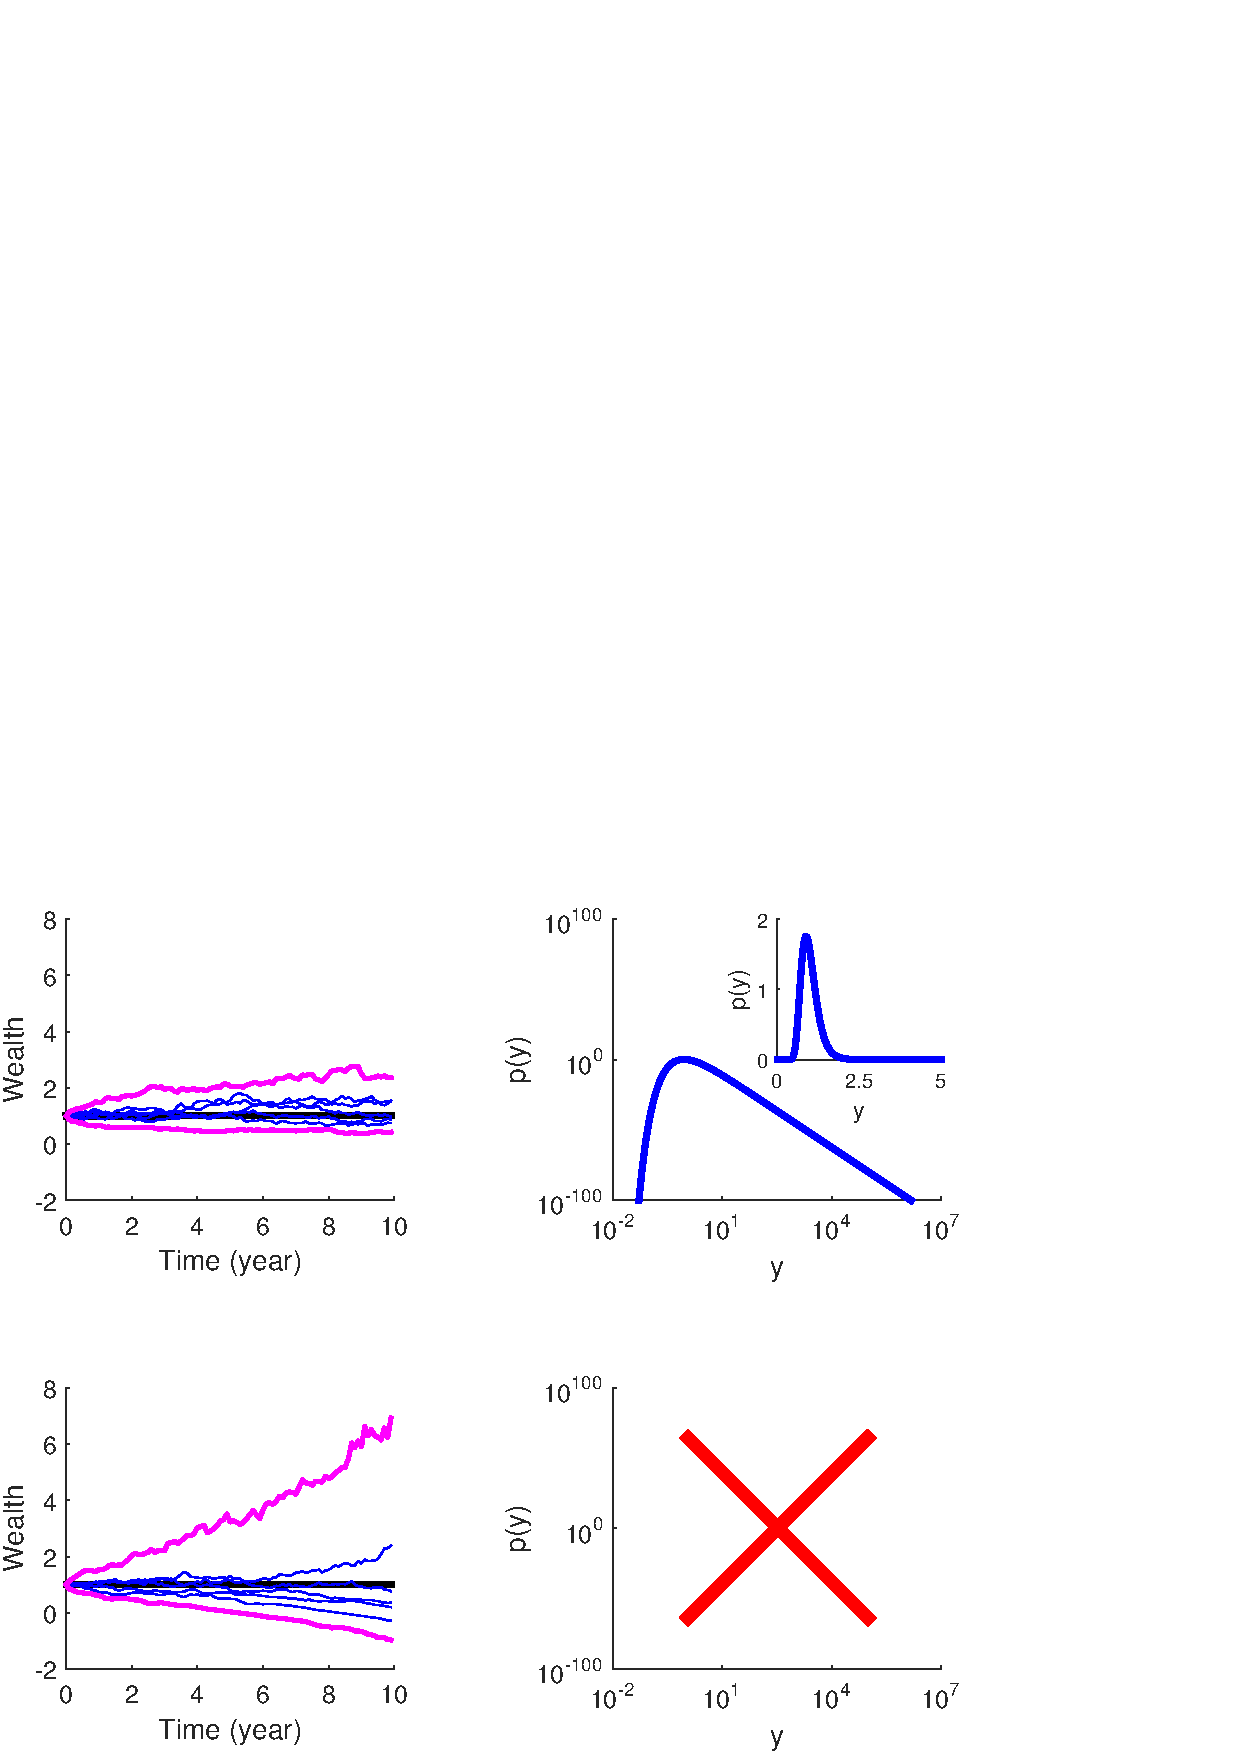
\includegraphics[height=9.3cm]{./chapter_3/figs/trajectories.pdf}
\caption{PEA and maximum in a finite ensemble of size $N=256$. {\bf \underline{Red line:}} expectation value $\ave{x(t)}$. 
{\bf \underline{Green line:}} exponential growth at the time-average growth rate. In the $T\to\infty$ limit all trajectories grow at this rate. 
{\bf \underline{Yellow line:}} contribution of the maximum value of any trajectory at time $t$ to the PEA.  
{\bf \underline{Blue line:}} PEA $\ave{x(t)}_N$.
{\bf \underline{Vertical line:}} Crossover -- for $t>t_c=\frac{2\ln N}{\sigma^2}$ the maximum begins to dominate the PEA (the yellow line approaches the blue line).
{\bf \underline{Grey lines:}} randomly chosen trajectories -- any typical trajectory soon grows at the time-average growth rate.  
{\bf \underline{Parameters:}} $N=256$, $\mu=0.05$, $\sigma=\sqrt{0.2}$.}
\flabel{trajectories}
\end{figure}
\FloatBarrier

\subsubsection{Our previous work on PEAs\seclabel{prevwork}}
In \cite{PetersKlein2013} we analysed PEAs of GBM analytically and numerically. Using \eref{GBM_sol} the PEA can be written as
\be
\ave{x}_N=\frac{1}{N} \sum_{i=1}^N \exp\left[ \left(\mu-\frac{\sigma^2}{2}\right) t + \sigma \gW_i(t) \right],
\elabel{PEA}
\ee
where $\left\{\gW_i(t)\right\}_{i=1\dots N}$ are $N$ independent realisations of the Wiener process. Taking the deterministic part out of the sum we re-write \eref{PEA} as
\be
\ave{x}_N=\exp\left[ \left(\mu-\frac{\sigma^2}{2}\right) t \right] \frac{1}{N} \sum_{i=1}^N \exp\left(t^{1/2} \sigma \xi_i\right),
\elabel{PEA_2}
\ee
where $\left\{\xi_i\right\}_{i=1\dots N}$ are $N$ independent standard normal variates.

We found that typical trajectories of PEAs grow at $\gex$ up to a time $t_c$ 
that is logarithmic in $N$, meaning $t_c\propto \ln N$. This is consistent with our sketch in \secref{sketch}. After this time, typical 
PEA-trajectories begin to deviate from expectation-value behavior, and eventually 
their growth rate converges to $g_t$. While the two limiting behaviours $N\to\infty$
and $t\to \infty$ can be computed exactly, what happens in between
is less straight-forward. The PEA is a random object outside these limits. 
In \cite{PetersKlein2013} we dealt with this issue numerically by creating a super-sample
of $S$ samples, each consisting of $N$ trajectories. In this way we were able to study the median of $\ave{x}_N(t)$, representing the behavior of typical trajectories.

A quantity of crucial interest to us is the exponential growth rate experienced by the PEA, 
\be
\gest(t,N) \equiv \frac{\ln(\ave{x(t)}_N)- \ln(x(0))}{t-0} = \frac{1}{t}\ln(\ave{x(t)}_N).
\elabel{gest}
\ee
In \cite{PetersKlein2013} we proved that the $t\to\infty$ limit for any (finite) 
$N$ is the same as for the case $N=1$, 
\be
\lim_{t\to\infty}\gest(t,N)=\mu-\frac{\sigma^2}{2}
\elabel{gest_2}
\ee
for all $N\geq1$. Substituting \eref{PEA_2} in \eref{gest} produces
\bea
\gest(t,N)&=&\mu-\frac{\sigma^2}{2}+\frac{1}{t} \ln\left(\frac{1}{N} \sum_{i=1}^N \exp( t^{1/2} \sigma \xi_i)\right)\\
&=&\mu-\frac{\sigma^2}{2}-\frac{\ln N}{t}+\frac{1}{t} \ln\left(\sum_{i=1}^N \exp( t^{1/2} \sigma \xi_i)\right).
\elabel{gest_4}
\eea

We didn't look in \cite{PetersKlein2013} at the expectation value of $\gest(t,N)$ for finite time and finite samples, but it's an interesting object that depends on $N$ and $t$ but is not stochastic. Note that this is not $\gest$ of the expectation value, 
which would be the $N\to\infty$ limit of \eref{gest}. Instead it is the 
$S\to\infty$ limit,
\be
\ave{\gest(t,N)} = \frac{1}{t}\ave{\ln(\ave{x(t)}_N)} = f(N,t),
\elabel{gest_3}
\ee
where, as in \secref{sketch}, $\ave{\cdot}$ without subscript refers to the average over all possible samples, \ie $\lim_{S\to\infty}\ave{\cdot}_{S}$. The last two terms in \eref{gest_4} suggest an exponential relationship between ensemble size and time. The final term is a tricky stochastic object on which the properties of the expectation value in \eref{gest_3} will hinge. This term will be the focus of our attention: the sum of exponentials of normal random variates or, equivalently, log-normal variates.


\subsubsection{Mapping to the random energy model}
Since the publication of \cite{PetersKlein2013} we have learned, thanks to discussions with J.-P.~Bouchaud, 
that the key object in \eref{gest_4} -- the sum of exponentials of normal random variates -- has been of
interest to the mathematical physics community since the 1980s. 

The reason for this is Derrida's random energy model \cite{Derrida1980,Derrida1981}. It is defined as follows. 
Imagine a system whose energy levels are $2^K=N$ random numbers $\xi_i$ (corresponding to $K=\ln N/\ln 2$ spins). This is
a very simple model of a disordered system, such as a spin glass, the idea being that the system is so complicated
that we ``give up'' and just model its energy levels as realizations of a random variable. (We denote the number 
of spins by $K$ and the number of resulting energy levels by $N$, whereas Derrida uses $N$ for the number of spins).
The partition function is then
\be
Z=\sum_{i=1}^N \exp\left(\beta J\sqrt{\frac{K}{2}}\xi_i\right),
\elabel{Z}
\ee
where the inverse temperature, $\beta$, is measured in appropriate units, and the scaling in $K$ is chosen
so as to ensure an extensive thermodynamic limit \cite[p.~79]{Derrida1980}. $J$ is a constant that will be determined below.
The logarithm of the partition function gives the Helmholtz free energy, 
\bea
F&=&-\frac{\ln Z}{\beta}\\
&=&-\frac{1}{\beta}  \ln\left[\sum_{i=1}^N \exp\left(\beta J \sqrt{\frac{K}{2}}\xi_i\right)\right].
\elabel{F}
\eea

Like the growth rate estimator in \eref{gest}, this involves a sum of 
log-normal variates and, indeed, we can rewrite \eref{gest_4} as
\be
\gest=\mu-\frac{\sigma^2}{2}-\frac{\ln N}{t}-\frac{\beta F}{t},
\elabel{gest_5}
\ee
which is valid provided that
\be
\beta J \sqrt{\frac{K}{2}}=\sigma t^{1/2}.
\elabel{map}
\ee
\Eref{map} does not give a unique mapping between the parameters of our GBM, $(\sigma, t)$, and the parameters of the REM, $(\beta, K, J)$. Equating (up to multiplication) the constant parameters, $\sigma$ and $J$, in each model gives us a specific mapping:
\be
\sigma=\frac{J}{\sqrt{2}} \quad \text{and} \quad t^{1/2} = \beta\sqrt{K}.
\elabel{choice_1}
\ee



The expectation value of $\gest$ is interesting. The only random object
in \eref{gest_5} is $F$. Knowing $\ave{F}$ thus amounts to knowing $\ave{\gest}$.
In the statistical mechanics of the random energy model $\ave{F}$ is of key
interest and so much about it is known. We can use this knowledge
thanks to the mapping between the two problems.

Derrida identifies a critical temperature,
\be
\frac{1}{\beta_c} \equiv \frac{J}{2\sqrt{\ln 2}},
\elabel{beta_c}
\ee
above and below which the expected free energy scales differently with $K$ and $\beta$. This maps to a critical time scale in GBM,
\be
t_c = \frac{2\ln N}{\sigma^2},
\elabel{t_c}
\ee
with high temperature ($1/\beta>1/\beta_c$) corresponding to short time ($t<t_c$) and low temperature ($1/\beta<1/\beta_c$) corresponding to long time ($t>t_c$). Note that $t_c$ in \eref{t_c} scales identically with $N$ and $\sigma$ as the transition time, \eref{short_t}, in our sketch.

In \cite{Derrida1980}, $\ave{F}$ is computed in the high-temperature (short-time) regime as
\bea
\ave{F}&=&E-S/\beta \\
&=&-\frac{K}{\beta} \ln2 - \frac{\beta K J^2}{4},
\elabel{F_2}
\eea
and in the low-temperatures (long-time) regime as
\be
\ave{F}=-KJ\sqrt{\ln 2}.
\elabel{F_3}
\ee

\underline{Short time}\\
We look at the short-time behavior first (high $1/\beta$, \eref{F_2}).
The relevant computation of the entropy $S$ in \cite{Derrida1980} 
involves replacing the number of energy levels
$n(E)$ by its expectation value $\ave{n(E)}$. This is justified because
the standard deviation of this number is $\sqrt{n}$ and relatively small
when $\ave{n(E)}>1$, which is the interesting regime in Derrida's case. 

For spin glasses, the expectation value of $F$ is interesting, supposedly, 
because the system may be self-averaging and can be thought of as an
ensemble of many 
smaller sub-systems that are essentially independent. The macroscopic
behavior is then given by the expectation value.

Taking expectation values and substituting from \eref{F_2} in \eref{gest_5} we find
\be
\ave{\gest}^{\text{short}}=\mu-\frac{\sigma^2}{2}+\frac{1}{t} \frac{K J^2}{4T^2}.
\elabel{gest_6}
\ee
From \eref{map} we know that $t=\frac{KJ^2}{2\sigma^2T^2}$, which we substitute, to find
\be
\ave{\gest}^{\text{short}}=\mu,
\elabel{gest_7}
\ee
which is the correct behavior in the short-time regime.

\underline{Long time}\\
Next, we turn to the expression for the long-time regime (low temperature, \eref{F_3}). 
Again 
taking expectation values and substituting, this time from \eref{F_3} in \eref{gest_5}, we find
for long times
\be
\ave{\gest}^{\text{long}}=\mu-\frac{\sigma^2}{2}-\frac{\ln{N}}{t}+\sqrt{\frac{2\ln N}{t}}\,\sigma,
\elabel{gest_8}
\ee
which has the correct long-time asymptotic behavior.
The form of the correction to the time-average growth rate
in \eref{gest_8} is consistent with \cite{PetersKlein2013} and \cite{Redner1990}, where
it was found that approximately $N=\exp(t)$ systems are required for ensemble-average
behavior to be observed for a time $t$, so that the parameter $\ln N/t$ controls
which regime dominates -- if the parameter is small, then \eref{gest_8} indicates that the
long-time regime is relevant.

\Fref{1} is a direct comparison between the results derived
here, based on \cite{Derrida1980}, and numerical results using the same parameter 
values as in \cite{PetersKlein2013}, namely $\mu=0.05, \sigma=\sqrt{0.2}, N=256$ and $S=10^5$.


Notice that $\ave{\gest}$ is not the (local)
time derivative $\frac{\partial}{\partial t}\ave{\ln(\ave{x}_N)}$, but a time-average growth rate, $\ave{\frac{1}{t}\ln\left( \frac{\ave{x(t)}_N}{\ave{x(0)}_N}\right)}$. 
In \cite{PetersKlein2013} we used a notation that we've stopped using since then because it
caused confusion -- $\ave{g}$ there denotes the growth rate of the expectation value, which 
is not the expectation value of the growth rate. 



It is remarkable that the expectation value $\ave{\gest(N,t)}$ so closely reflects the
median, $q_{0.5}$, of $\ave{x}_N$, in the sense that
\be
q_{0.5}(\ave{x(t)}_N) \approx \exp \left(\ave{\gest(N,t)}t\right).
\elabel{quant_ave}
\ee
In \cite{PetersGell-Mann2016} it was discussed in detail that 
$\gest(1,t)$ is an ergodic observable for \eref{GBM}, in the sense that 
$\ave{\gest(1,t)}=\lim_{t\to\infty} \gest$. The relationship in \eref{quant_ave}
is far more subtle. The typical behavior of GBM PEAs 
is complicated outside the limits $N\to\infty$ or $t\to\infty$, in the sense that growth rates are 
time dependent here. This complicated behavior is well represented by an 
approximation that uses physical insights into spin glasses. Beautiful!

\begin{figure}
\centering
\includegraphics[height=9.3cm]{./chapter_3/figs/PEA.pdf}
\caption{Lines are obtained by exponentiating the various exponential 
growth rates. {\bf \underline{Blue line:}} $\ave{\ave{\gest}_{256}}_{10,000}$ is the numerical mean 
(approximation of the expectation value) 
over a super-ensemble of $S=10,000$ samples of $\gest$ estimated in sub-ensembles of $N=256$ GBMs each. 
{\bf \underline{Green line:}} median in a super-ensemble of $S$ samples of $\gest$, each estimated in sub-ensembles of size $N$. 
{\bf \underline{Yellow line:}} \eref{Ito_sums} is an exact expression for $d\ave{\ln\ave{x}_N}$, derived using \Ito calculus. We evaluate the expression by Monte Carlo, and integrate, $\ave{\ln\ave{x}_N}=\int_{0}^{t} d\ave{\ln\ave{x}_N}$. Exponentiation yields the yellow line. 
{\bf \underline{Red line:}} short-time behavior, based on the random energy model, \eref{gest_7}.
{\bf \underline{Purple line:}} long-time behavior, based on the random energy model, \eref{gest_8}. {\bf \underline{Vertical line:}} Crossover between the regimes at $t_c=\frac{2\ln N}{\sigma^2}$, corresponding to $\beta_c=\frac{2(\ln 2)^{1/2}}{J}$.
{\bf \underline{Parameters:}} $N=256$, $S=10,000$, $\mu=0.05$, $\sigma=\sqrt{0.2}$.}
\flabel{1}
\end{figure}
\FloatBarrier
%

\subsubsection{Another route via \Ito calculus}
Another way to find the expectation value of PEA growth rates, \eref{gest_3}, 
is to compute $\ave{d\ln \ave{x}_N}$ using \Ito calculus. We compute this directly, without 
invoking the random energy model. To apply \Ito calculus, 
we will need the first two partial derivatives of $d\ln\ave{x}_N$ with respect to $x_i$.
\be
\frac{\partial \ln \ave{x}_N}{\partial x_i}=\frac{1}{N\ave{x}_N}
\ee
and
\be
\frac{\partial^2 \ln \ave{x}_N}{\partial x_i^2}=-\frac{1}{N^2\ave{x}_N^2}
\ee
Now, Taylor-expanding $d \ln \ave{x}_N$ we find
\bea
d \ln \ave{x}_N&=&\sum_i \frac{\partial \ln \ave{x}_N}{\partial x_i} dx_i+\frac{1}{2}\sum_i \sum_j \frac{\partial^2 \ln \ave{x}_N}{\partial x_i \partial x_j} dx_i dx_j+ \ldots\\
&\approx&\frac{1}{N\ave{x}_N} \sum_i dx_i-\frac{1}{2N^2\ave{x}_N^2}\sum_i \sum_j dx_i dx_j.
\eea
The double-sum can be split into `diagonal' ($i=j$) terms and cross-terms as
\be
\frac{1}{N\ave{x}_N}\sum_i x_i(\mu dt + \sigma dW_i) -\frac{1}{2N^2\ave{x}_N^2 }\left(\sum_i  dx_i^2 + \sum_{j}\sum_{i \neq j}dx_i dx_j\right)\hspace{.6cm}
\ee
Parts of the cross-terms are negligible because they are of order $dt^2$ and the rest vanishes when taking the expectation value, 
as we see by writing out one cross term
\be
dx_i dx_j=x_i x_j (\mu^2 dt^2+\mu\sigma dt dW_i+\mu \sigma dt dW_j + \sigma^2 dW_i dW_j).
\ee
We therefore drop these terms now, as we take the expectation value, using the Wiener identity $\ave{dW_i^2}=dt$ for the final term
\bea
\ave{d \ln \ave{x}_N}&=&\ave{\mu dt -\frac{1}{2N^2\ave{x}_N^2}\sum_i x_i^2 (\mu^2 dt^2 + \sigma^2 dt)} \\
&=&\mu dt   -\ave{\frac{1}{2} \sigma^2 \frac{\ave{x^2}_N}{N\ave{x}_N^2}} dt + O(dt^2).
\eea
Discarding terms of higher-than-first order in $dt$ and re-writing the last term as a fraction of sums, we thus have 
\bea
\frac{\ave{d \ln \ave{x}_N}}{dt}&=&\mu -\frac{1}{2} \sigma^2  \ave{\frac{\frac{1}{N}\sum_i x_i^2}{N\left(\frac{1}{N}\sum_i x_i\right)^2}}  \\
&=&\mu -\frac{1}{2} \sigma^2  \ave{\frac{\sum_i x_i^2}{\left(\sum_i x_i\right)^2}} \elabel{Ito_sums}
\eea
This expression has the correct behaviour: for short times, all $x_i$ are essentially identical, 
and the second term is $-\frac{1}{2}\sigma^2 \frac{1}{N}$, which is negligible if $N$ is large. So, for short times
we see expectation-value behaviour. For long times, the largest $x_i$ will dominate both the numerator and the denominator, and we have
$-\frac{1}{2}\sigma^2$: the full \Ito correction is felt for long times.

\subsubsection{Discussion}
The \Ito result is exact. A Monte-Carlo estimate of \eref{Ito_sums} (which is easy to obtain) is 
shown in \fref{1} (yellow line). This agrees well with numerical observations.
The approximations from the random energy model have the right shape and asymptotic behavior, 
though they're not on the same scale as the median PEA. This is, of course, not surprising because
these estimates are not designed to coincide with the median PEA. Quantitatively they are closer to 
a higher quantile of the distribution of PEAs. An intriguing question is this: is our computation 
using \Ito calculus helpful to compute the expected free energy of the random energy model? 

\subsection{Cooperation}
\seclabel{Cooperation}
Under multiplicative growth, fluctuations are undesirable because they reduce 
time-average growth rates. In the long run, wealth $x_1(t)$ with noise term 
$\sigma_1$ will outperform wealth $x_2(t)$ with a larger 
noise term $\sigma_2>\sigma_1$, in the sense that 
\be
\gt(x_1) > \gt(x_2)
\ee
with probability 1.

For this reason it is desirable to reduce fluctuations. One protocol that achieves this is 
resource pooling and sharing. In \secref{Every_man} we explored the world created 
by the model of independent GBMs. This is a world where everyone experiences the 
same long-term growth rate. We want to explore the effect of the invention of 
cooperation. As it turns out cooperation increases growth rates, and this is a 
crucial insight. 

Suppose two individuals, $x_1(t)$ and $x_2(t)$ decide to meet up every Monday, put all 
their wealth on a table, divide it in two equal amounts, and go back to their business, \ie
they submit their wealth to our toy dynamic \eref{GBM}. How 
would this operation affect the dynamic of the wealth of these two individuals?

 Consider a discretized version of \eref{GBM}, such as would be used in a numerical simulation. The non-cooperators grow according to
 \bea
 \d x_i(t) & = & x_i(t) \left[\mu \dt + \sigma \sqrt{\dt}\,\xi_i\right], \elabel{discrete_nonc_grow} \\
 x_i(t+\dt) & = & x_i(t) + \d x_i(t), \elabel{discrete_nonc_coop}
 \eea
 where $\xi_i$ are standard normal random variates, $\xi_i\sim \mathcal{N}(0,1)$.

We imagine that the two previously non-cooperating entities, with resources $x_1(t)$ and $x_2(t)$, cooperate to produce two entities, whose resources we label $x^c_1(t)$ and $x^c_2(t)$ to distinguish them from the non-cooperating case. We envisage equal sharing of resources, $x^c_1=x^c_2$, and introduce a cooperation operator, $\oplus$, such that
 \be
 x_1 \oplus x_2 = x^c_1 + x^c_2.
 \ee
 
 In the discrete-time picture, each time step involves a two-phase process. First there is a growth phase, analogous to \eref{GBM}, in which each cooperator increases its resources by
 \be
 \d x^c_i(t) = x^c_i(t)\left[\mu\dt + \sigma\sqrt{\dt}\,\xi_i\right].
 \elabel{discrete_coop_grow}
 \ee
 This is followed by a cooperation phase, replacing \eref{discrete_nonc_coop}, in which resources are pooled and shared equally among the cooperators:
 \be
 x^c_i(t+\dt) = \frac{ x^c_1(t) + \d x^c_1(t) + x^c_2(t) + \d x^c_2(t)}{2}.
 \elabel{discrete_coop_coop}
 \ee
 
 \begin{figure}
 \centering
 \begin{picture}(300,230)(60,0)
 \put(-20,0){\includegraphics[width=470pt]{./chapter_3/figs/blobs.pdf}}
 \put(0,145){$x^c_1(t)$}
 \put(48,147){\vector(1,0){45}}
 \put(0,40){$x^c_2(t)$}
 \put(48,40){\vector(1,0){75}}
 %
 \put(115,145){$x^c_1(t)+\d x^c_1(t)$}
 \put(200,147){\vector(3,-2){30}}
 \put(138,46){$x^c_2(t)$}
 \put(130,34){$+\d x^c_2(t)$}
 \put(173,45){\vector(3,2){50}}
 %
 \put(255,100){$x^c_1(t)+\d x^c_1(t)$}
 %
 \put(250,85){$+ x^c_2(t)+\d x^c_2(t)$}
 \put(335,75){\vector(3,-2){30}}
 \put(335,117){\vector(3,2){30}}
 %
 \put(385,145){$x^c_1(t+\dt)$}
 \put(385,40){$x^c_2(t+\dt)$}
 %
 \put(448,147){\vector(1,0){25}}
 \put(448,40){\vector(1,0){25}}

 \put(476,144.5){$\cdots$}
 \put(476,37.5){$\cdots$}
 % AA extra arrows
 \put(-47,117){\vector(3,2){25}}
 \put(-47,75){\vector(3,-2){25}}
 \put(-62,114){$\cdots$}
 \put(-62,73){$\cdots$}
 %
 \put(50,207.5){\large{Grow}}

 \put(215,190){$\overbrace{\text{Pool} \hspace{3cm}\text{Share}}^{\text{\large{Cooperate}}}$}

 \end{picture}
 \caption{Cooperation dynamics. Cooperators start each time step with equal resources, then they {\it grow} independently 
 according to \eref{discrete_coop_grow}, then they {\it cooperate} by {\it pooling} resources and {\it sharing} them equally, 
 then the next time step begins. 
  }
 \flabel{dynamics}
 \end{figure}
 

 %Analysis
 With this prescription both cooperators and their sum experience the following dynamic:
 \be
 (x_1 \oplus x_2)(t+\dt) =
 (x_1 \oplus x_2)(t) \left[1 + \left(\mu \dt + \sigma \sqrt{\dt} \, \frac{\xi_1 + \xi_2}{2}\right)\right].
 \elabel{discrete_cooperate}
 \ee
 For ease of notation we define
 \be
 \xi_{1\oplus2}=\frac{\xi_1+\xi_2}{\sqrt{2}},
 \ee
 which is another standard Gaussian, $\xi_{1\oplus2} \sim \mathcal{N}(0,1)$. Letting the time
 increment $\dt \to 0$ we recover an equation of the same form as
 \eref{GBM} but with a different fluctuation amplitude,
 \begin{equation}
 d(x_1 \oplus x_2) = (x_1 \oplus x_2)\left(\mu dt +\frac{\sigma}{\sqrt{2}} dW_{1\oplus2}\right).
 \end{equation}
 
The expectation values of a non-cooperator, $\ave{x_1(t)}$, and a corresponding cooperator,
$\ave{x^c_1(t)}$, are identical. Based on expectation values, we thus cannot 
 see any benefit of cooperation. Worse still, immediately after the growth phase, the 
 better-off entity of a cooperating pair, $x^c_1(t_0)>x^c_2(t_0)$, say, would increase its expectation value from 
$\frac{x^c_1(t_0)+x^c_2(t_0)}{2}\exp(\mu (t-t_0))$ to $x^c_1(t_0)\exp(\mu (t-t_0))$
by breaking the cooperation. But it would be foolish to act on the basis of this analysis --
the short-term gain from breaking cooperation is a one-off, and is dwarfed by the long-term
multiplicative advantage of continued cooperation. 
An analysis based on expectation values finds that there is no reason for 
cooperation to arise, and that if it does arise there are good reasons for it to end, 
\ie it will be fragile. Because expectation values are inappropriately used to evaluate 
future prospects, the observation of widespread cooperation constitutes a conundrum. 

%Solution of the cooperation conundrum
The solution of the conundrum comes from considering the time-average
growth rate. The non-cooperating entities grow at $g_{t}(x_i)=\mu-\frac{\sigma^2}{2}$, 
whereas the cooperating unit benefits from a reduction of the amplitude of relative 
fluctuations and grows at $g_{t}(x_1\oplus x_2)=\mu-\frac{\sigma^2}{4}$, 
and we have
\begin{equation}
g_{t}(x_1\oplus x_2)>g_{t}(x_i)
\end{equation}
for any non-zero noise amplitude. Imagine a world where cooperation does not exist, 
just like in \secref{Every_man}. Now introduce into this world two individuals who have 
invented cooperation -- very quickly this pair of individuals will be vastly more wealthy than
anyone else. To keep up, others will have to start cooperating. The effect is illustrated 
in \fref{cooperate} by direct simulation of
\eref{discrete_nonc_grow}--\eref{discrete_nonc_coop} and \eref{discrete_cooperate}.

\begin{figure}
\begin{picture}(200,300)(0,0)
\put(-35,-135){\includegraphics[width=440pt]{./chapter_3/figs/cooperate.pdf}}
\end{picture}
\caption{Typical trajectories for two non-cooperating (green) entities and for the 
corresponding cooperating unit (blue).
Over time, the noise reduction for the cooperator leads to faster growth. Even without
effects of specialisation or the emergence of new function, 
cooperation pays in the long run. The black thin line shows the average of the 
non-cooperating entities. While in the logarithmic vertical scale the average traces
the more successful trajectory, it is far inferior to the cooperating unit. 
In a very literal mathematical sense the whole, $(x_1 \oplus x_2)(t)$, is more than the sum of its
parts, $x_1(t)+x_2(t)$. The algebra of cooperation is not merely that of summation.}
\flabel{cooperate}
\end{figure}

Imagine again the pair of cooperators outperforming all of their peers. Other
entities will have to form pairs to keep up, and the obvious next step is for larger
cooperating units to form -- groups of 3 may form, pairs of pairs, cooperation 
clusters of $n$ individuals, and the larger the cooperating group the closer the
time-average growth rate will get to the expectation value.
For $n$ cooperators, $x_1\oplus x_2 ... \oplus x_n$ the spurious drift term is 
$-\frac{\sigma^2}{2n}$, so that the time-average growth approaches 
expectation-value growth for large $n$. The approach to this upper bound as 
the number of cooperators increases favours the formation of social structure. 

We may generalise to different drift 
terms, $\mu_i$, and noise amplitudes, $\sigma_i$, for different individual entities. 
Whether cooperation is beneficial in the long run for any
given entity depends on these parameters as follows. Entity 1 
will benefit from cooperation with entity 2 if 
\be
\mu_1-\frac{\sigma_1^2}{2}<\frac{\mu_1+\mu_2}{2}-\frac{\sigma_1^2+\sigma_2^2}{8}.
\ee
We emphasize that this inequality may be satisfied also if the expectation value
of entity 1 grows faster than the expectation value of entity 2, \ie if
$\mu_1>\mu_2$. An analysis of expectation values, again, is utterly misleading:
the benefit conferred on entity 1 due to the fluctuation-reducing effect of 
cooperation may outweigh the cost of having to cooperate with an entity with
smaller expectation value.
 
Notice the nature of the Monte-Carlo simulation in \fref{cooperate}. No ensemble
is constructed. Only individual trajectories are simulated and run for a time that is 
long enough for statistically significant features to rise above the noise. This method
teases out of the dynamics what happens over time. The significance of any observed 
structure -- its epistemological meaning -- is immediately clear: this is what happens over time
for an individual system (a cell, a person's wealth, {\it etc.}). Simulating an ensemble
and averaging over members to remove noise does not tell the same story. The resulting
features may not emerge over time. They are what happens on average in an ensemble, 
but -- at least for GBM -- this is not what happens to the individual with probability 1. For instance the 
 pink dashed line in \fref{cooperate} is the ensemble average of $x_1(t)$, $x_1(t)$, 
 and $(x_1 \oplus x_2)(t)/2$, and it has nothing to do with what happens 
 in the individual trajectories over time.

When judged on expectation values, the apparent futility of cooperation is unsurprising
because expectation values are the result for infinitely 
many cooperators, and adding further cooperators cannot improve on this.

In our model the advantage of cooperation, and hence the emergence
of social structure in the broadest sense -- is purely a non-linear 
effect of fluctuations -- cooperation reduces the magnitude of 
fluctuations, and over time (though not in expectation) this implies faster growth. 


Another generalisation is partial cooperation -- entities may share only
a proportion of their resources, resembling taxation and redistribution. We discuss this in
the next section.
\FloatBarrier

\subsection{\seclabel{Taxation}Taxation}
In \secref{Every_man} we created a world of independent GBMs; in \secref{Cooperation} 
we introduced to this world
the invention of cooperation and saw that it increases long-time growth for those who participate
in resource-pooling and sharing. In this section we study what happens if a large number
of individuals pool and share a small fraction of their resources, which is reminiscent of taxation
and redistribution carried out in a large population. We will find that while cooperation for 2 individuals
increases their growth rates, sufficient cooperation in a large population
has two related effects. Firstly, everyone's wealth grows asymptotically at a rate close to that of
the expectation value. Secondly, wealth condensation and the divergence of inequality 
no longer occur.

We introduce a model that applies a flat wealth tax rate and every individual, irrespective of his 
wealth, receives the same benefit from the collected tax, in absolute terms. This mimicks the
actions of a central agency that collects each year from everyone 1\% of his wealth and pays 
1-$N^\text{th}$ of the total collected amount to each individual. A similar model will be 
used for income tax, see \eref{isde} in \secref{Income_tax}. 

Of course this isn't how taxation works in reality -- wealth taxes are usually only collected in 
the form of inheritance tax and sometimes property or land tax; often progressive rates are 
applied, and how tax takings are actually redistributed is very unclear. 
Who benefits from government activity? Infrastructure is built, benefits payments made, 
healthcare and education provided, a legal system is maintained of courts that can 
enforce contracts and enable corporate structures, police and an army may provide security. 
Individuals will benefit from these different aspects to very different degrees. Our model 
ignores this and lets everyone benefit equally.

Despite the simplicity of the setup the following important feature emerges:
there is a critical tax rate. This qualitative result applies both to income tax and to wealth tax.

\definition{ {\bf Critical tax rate}\\
Below the critical tax rate the variance of rescaled wealth increases indefinitely. 
Above the critical tax rate it stabilizes to an asymptotic value in the limit $t\to\infty$.
}

\Secref{Cooperation} was concerned with growth, here we are concerned with inequality. 
We will therefore work with the rescaled wealth, $y$, introduced in \eref{rescaled}. \Eref{GBM} defines the 
dynamic of $x$. From it we can find the dynamic for $f(x)=y$ using \Ito calculus
\bea
df &=& \frac{\partial f}{\partial x} dx + \frac{\partial f}{\partial t} + \frac{1}{2} \frac{\partial^2 f}{\partial x^2} dx^2\\
=dy&=& -\mu y dt + \frac{y}{x} dx\\
&=&y \sigma dW.
\eea



\subsubsection{Wealth tax}
\seclabel{Wealth_tax}
We investigate the situation where each individual's wealth is taxed at a rate of $0\leq\tau\leq1$ per unit time, 
and the total tax thus raised is redistributed equally among the population. This is modelled by the stochastic wealth process,
\be
dx = x[(\mu-\tau)\,dt + \sigma\,dW] + \tau\ave{x}_N dt,
\elabel{wsde}
\ee
which is a modified version of \eref{GBM} -- the term $-\tau x dt$ was added to represent tax 
collection, and the term $+\tau \ave{x}_N dt$ to represent redistribution of collected tax.
To make the model more tractable we consider the case $N \to \infty$, which replaces the finite-ensemble 
average by the expectation value, $\ave{x}_N \to \ave{x}$. The finite ensemble size has important effects but 
we will not discuss them here.
Total wealth is conserved by the taxation and redistribution process in this model, 
and the expectation value is unaffected, $\ave{x(t)}=\ave{x_0}e^{\mu t}$, just as for GBM without taxation, \eref{exp_x}. 
We are again interested in rescaled wealth, $y=\frac{x}{\ave{x}}=x e^{-\mu t}$ (\eref{rescaled}), whose dynamic we derive using the chain rule
\bea
dy &=& \frac{\partial y}{\partial t}\,dt + \frac{\partial y}{\partial x}\,dx + \frac{1}{2} \frac{\partial^2 y}{\partial x^2} \,dx^2 \\
&=& -\mu y\,dt + \frac{1}{x}\,dx \elabel{ysde} \\
&=& y(-\tau dt+ \sigma dW)+\tau dt.
\eea
The first moment of $y$ is trivially $1$,
\be
\ave{y}=\ave{\frac{x}{\ave{x}}}=1.
\ee
We compute the dynamic of the second moment of $y$, to first order in $dt$, using the chain rule again,
\bea
d(y^2)&=& \frac{\partial (y^2)}{\partial t}\,dt + \frac{\partial (y^2)}{\partial y}\,dy + \frac{1}{2} \frac{\partial^2 (y^2)}{\partial y^2} \,(dy)^2\\
&=&2y dy + (dy)^2\\
&=& 2y^2(-\tau dt+ \sigma dW)+2y\tau dt +y^2\sigma^2 dt.
\eea
Taking expectation values yields 
\bea
\ave{dy^2}&=& \ave{-2y^2(-\tau dt+ \sigma dW)+2y\tau dt -y^2\sigma^2dt}\\
=d\ave{y^2}&=&(\sigma^2-2\tau) \ave{y^2} dt + 2\tau dt.
\eea
This equation is an inhomogeneous first-order ordinary differential equation for 
the second moment. Perhaps it's more recognizable when written in standard form as
\be
\left(\frac{d}{dt}- (\sigma^2-2\tau)\right)\ave{y^2}= 2\tau.
\elabel{ODE2}
\ee
Such equations are solvable using the method of integrating factors, see \eg \cite[Chpater 1.5]{BenderOrszag1978}.
The solution of the dynamic \eref{ODE2} is the second moment 
of the distribution of rescaled wealth as a function of time, namely
\be
\ave{y^2} = \frac{2\tau}{2\tau-\sigma^2} + \left(\ave{y_0^2} - \frac{2\tau}{2\tau-\sigma^2}\right) e^{-(2\tau-\sigma^2)t}.
\ee
This can be rewritten in terms of the variance of rescaled wealth, $V=\ave{y^2}-1$, as
\be
V(t) = V_\infty + (V_0 - V_\infty) e^{-(2\tau-\sigma^2)t},
\elabel{wvar}
\ee
where $V_0$ is the initial variance and
\be
V_\infty \equiv \frac{\sigma^2}{2\tau-\sigma^2}.
\ee
$V$ converges in time to the asymptote, $V_\infty$, provided the exponential in \eref{wvar} is decaying. This can be expressed as a condition on $\tau$,
\be
\boxed{
\tau > \tau_c \equiv \frac{\sigma^2}{2},
}
\elabel{wstab}
\ee
which defines the critical tax rate, $\tau_c$. Above this critical tax rate, $\tau>\tau_c$, the 
variance of the rescaled-wealth distribution stabilises. Below it, the variance grows beyond all bounds.
We believe that the divergence or convergence of the variance signals an important change
in systemic behavior, but we hasten to point out the following caveat: a finite second moment 
does not guarantee finiteness of higher moments. A deeper analysis of ODEs of the type of 
\eref{ODE2}, which we don't reproduce here, reveals that any finite wealth tax rate implies
that all moments of order $n>\frac{2\tau}{\sigma^2}+1$ diverge. Under the flat 
wealth tax investigated here, the wealth distribution never fully stabilizes. In the language often
used by economists in this debate, an ergodic wealth distribution does not exist for our model.

Caveats aside, \eref{wvar} also allows us to identify a characteristic timescale over 
which the variance stabilises for supercritical taxation,
\be
T_s = \frac{1}{2\tau-\sigma^2}.
\ee
$\tau_c$ may be viewed as the tax rate at which $T_s$ diverges.

Numerical simulations confirm that the above analytical results are informative for finite ensembles. 
\fref{var_wealth} compares the 
evolution of the empirical variance of the rescaled wealths of $N=10^4$ realisations of the 
stochastic wealth process in \eref{wsde} with the theoretical result for the infinite ensemble 
in \eref{wvar}. Parameter values were $\mu=0.05$, $\sigma^2=0.02$, and $\tau=0.1$ per 
unit time, of which the first two are realistic for a time unit of one year \cite{PetersAdamou2013} 
(assuming individual wealth processes share parameters with stock market indices). The 
differences are finite-sample effects.
\begin{figure}
\bc
\includegraphics[width=0.8\textwidth]{./chapter_3/figs/var_wealth.pdf}
\caption{Wealth tax. The empirical variance of the rescaled wealths of $N=10^4$ realisations of 
\eref{wsde} with uniformly-distributed initial wealths (red); the theoretical variance for the infinite 
ensemble, $V(t)$ (blue dashed); and the asymptotic theoretical variance, $V_\infty$ (black dotted). 
Parameter values are $\mu=0.05$, $\sigma^2=0.02$, and $\tau=0.1$ per unit time.}
\flabel{var_wealth}
\ec
\end{figure}
\fref{hist_wealth} shows the initial distribution of rescaled wealths, which was chosen to be uniform, 
and the final distribution at the end of the period shown in \fref{var_wealth}.
\begin{figure}
\bc
\includegraphics[width=0.8\textwidth]{./chapter_3/figs/hist_wealth.pdf}
\caption{Histograms of the initial (left) and final (right) empirical distributions of the rescaled 
wealth for the same realisations of \eref{wsde} used in \fref{var_wealth}.}
\flabel{hist_wealth}
\ec
\end{figure}

The simulated parameter values give a critical tax rate of 1\% pa. This is broadly in line 
with genuine annual wealth and property taxes in the few countries in which they are 
levied. Under the simulated tax rate of 10\% pa, the stabilisation time is $T_s\approx6$ 
years. It is hard to imagine a wealth tax of this magnitude being politically feasible in the 
real world. In our simple model, the tax rate could be set either to achieve convergence 
of inequality to a desired level, reflected by $V_\infty$, or over a desired timescale, 
represented by $T_s$.

It is interesting to connect this with the most widely levied wealth tax: the inheritance 
tax. In the UK this is levied at 40\% of the value of an individual's estate (above a 
certain threshold) upon death. We can surmise that an individual will typically hold 
most of his wealth for the human generation time of around 30 years, this being a 
sensible estimate of the time between inheriting or otherwise accumulating his wealth 
and passing it on. Using our plausible parameter values, an inheritance tax of 40\% 
corresonds to an annually compounded wealth tax of $1-(0.6)^{1/30} \approx 1.7\%$ 
pa and a stabilisation time of around 70 years. The former is close to and, notably, 
above the critical rate of 1\% pa, suggesting that variance stabilisation may be an 
influential criterion in the determination of our taxes.

\subsubsection{Income tax}
\seclabel{Income_tax}
In our very simple model, we have seen that a flat wealth tax can stabilize
the variance of the rescaled-wealth distribution. In this section we show 
that in a similarly simple model an income tax can achieve the same result. 
We introduce a model of income tax under which a fraction, $0\leq\tau\leq1$, of 
each individual's determinsitic wealth increment, $\mu x\,dt$, is deducted and 
the total tax raised is redistributed equally. This is modelled by the stochastic wealth process,
\be
dx = x[\mu(1-\tau)\,dt + \sigma\,dW] + \mu\tau\ave{x}_N dt.
\elabel{isde}
\ee
Again, we consider the large-population limit $N\to\infty$, corresponding to the replacement 
$\ave{x}_N\to\ave{x}$. For positive drift, $\mu>0$, the deterministic increment, $\mu x\,dt$, is guaranteed to 
be positive. It can be thought of as the income derived from that individual's activities, 
such as employment, on which governments typically levy taxes. Note that $\tau$ in \eref{isde} is a dimensionless number, whereas it is
a rate of dimension ``per unit time'' in \eref{wsde}. The form of 
\eref{isde} is identical to \eref{wsde} with the parameter transformation 
$\tau\rightarrow\mu\tau$. Thus we can immediately deduce the dynamic for the rescaled wealth as
\be
dy = y(-\mu\tau\,dt + \sigma\,dW) + \mu\tau\,dt.
\elabel{itax}
\ee
The variance stabilisation condition analogous to \eref{wstab} becomes
\be
\boxed{
\tau > \tau_c \equiv \frac{\sigma^2}{2\mu}.
}
\elabel{icrit}
\ee
This defines the critical income tax, $\tau_c$, above which the variance converges to its asymptotic value,
\be
V_\infty = \frac{\sigma^2}{2\mu\tau-\sigma^2},
\ee
according to
\be
V(t) = V_\infty + (V_0 - V_\infty) e^{-(2\mu\tau-\sigma^2)t}.
\elabel{ivar}
\ee
Finally, the stabilisation time is
\be
T_s = \frac{1}{2\mu\tau - \sigma^2}.
\ee

\fref{var_income} compares the evolution of the empirical variance of the rescaled wealths of $10^4$ realisations of the stochastic wealth process in \eref{isde} with the theoretical result for the infinite ensemble. Parameter values were $\mu=0.05$ and $\sigma^2=0.02$ per unit time, and $\tau=0.45$. The latter is the UK's limiting income tax rate for large incomes, which will be the determining tax rate for variance stabilisation.
\begin{figure}
\bc
\includegraphics[width=0.8\textwidth]{./chapter_3/figs/var_income.pdf}
\caption{Income tax. The empirical variance of the rescaled wealths of $10^4$ realisations of \eref{isde} with uniformly-distributed initial wealths (red); the theoretical variance for the infinite ensemble, $V(t)$ (blue dashed); and the asymptotic theoretical variance, $V_\infty$ (black dotted). Parameter values are $\mu=0.05$ and $\sigma^2=0.02$ per unit time, and $\tau=0.45$.}
\flabel{var_income}
\ec
\end{figure}

The finite-sample deviations from the infinite-ensemble result are larger in \fref{var_income} 
than in \fref{var_wealth}. This is due entirely to the simulated parameter values: \eref{wsde} 
and \eref{isde} can be made equivalent by choosing different parameters. 
%Quantifying the scales of the finite-sample effects, and particularly their dependence 
%on $\tau$, would go some way towards illustrating the difference in the stabilisation 
%properties of the two taxation types under potentially realistic tax rates. This may be 
%a worthwile project.

\fref{hist_income} shows the initial distribution of rescaled wealths, which was chosen to be uniform, and the final distribution at the end of the period shown in \fref{var_income}.
\begin{figure}
\bc
\includegraphics[width=0.8\textwidth]{./chapter_3/figs/hist_income.pdf}
\caption{Histograms of the initial (left) and final (right) empirical distributions of the rescaled wealth for the same realisations of \eref{itax} used in \fref{var_income}.}
\flabel{hist_income}
\ec
\end{figure}
The distribution of wealths under income tax has an appreciably longer tail than under wealth tax. As before this is a function of the parameter choices. The simulated parameter values have a critical income tax rate of $\tau_c=0.2$ and a stabilisation time of $T_s=40$ years. Thus the UK sets its income tax at a level which, at least in this simple framework, has a variance stabilising effect.
\FloatBarrier
%
%\bibliographystyle{abbrv}
%\bibliography{./../bibliography}
%
%\end{document}